% !TeX document-id = {f19fb972-db1f-447e-9d78-531139c30778}
% !BIB program = biber

%\documentclass[handout]{beamer}
\documentclass[compress]{beamer}
\usepackage[T1]{fontenc}
\usetheme[block=fill,subsectionpage=progressbar,sectionpage=progressbar]{metropolis} 
\usepackage{graphicx}

\usepackage{wasysym}
\usepackage{etoolbox}
\usepackage[utf8]{inputenc}

\usepackage{pifont}

\usepackage{threeparttable}
\usepackage{subcaption}

\usepackage{tikz-qtree}
\usepackage{neuralnetwork}

\setbeamercovered{still covered={\opaqueness<1->{5}},again covered={\opaqueness<1->{100}}}


\usepackage{listings}

\lstset{
	basicstyle=\scriptsize\ttfamily,
	columns=flexible,
	breaklines=true,
	numbers=left,
	%stepsize=1,
	numberstyle=\tiny,
	backgroundcolor=\color[rgb]{0.85,0.90,1}
}



\lstnewenvironment{lstlistingoutput}{\lstset{basicstyle=\footnotesize\ttfamily,
		columns=flexible,
		breaklines=true,
		numbers=left,
		%stepsize=1,
		numberstyle=\tiny,
		backgroundcolor=\color[rgb]{.7,.7,.7}}}{}


\lstnewenvironment{lstlistingoutputtiny}{\lstset{basicstyle=\tiny\ttfamily,
		columns=flexible,
		breaklines=true,
		numbers=left,
		%stepsize=1,
		numberstyle=\tiny,
		backgroundcolor=\color[rgb]{.7,.7,.7}}}{}


% color-coded listings; replace those above 
\usepackage{xcolor}
\usepackage{minted}
\definecolor{listingbg}{rgb}{0.87,0.93,1}
\setminted[python]{
	frame=none,
	framesep=1mm,
	baselinestretch=1,
	bgcolor=listingbg,
	fontsize=\scriptsize,
	linenos,
	breaklines
	}


\usepackage[american]{babel}
\usepackage{csquotes}
\usepackage[style=apa, backend = biber]{biblatex}
\renewcommand*{\bibfont}{\tiny}


\usepackage{tikz}
\usetikzlibrary{shapes,arrows,matrix}
\usepackage{multicol}

\usepackage{subcaption}

\usepackage{booktabs}
\usepackage{graphicx}



\makeatletter
\setbeamertemplate{headline}{%
	\begin{beamercolorbox}[colsep=1.5pt]{upper separation line head}
	\end{beamercolorbox}
	\begin{beamercolorbox}{section in head/foot}
		\vskip2pt\insertnavigation{\paperwidth}\vskip2pt
	\end{beamercolorbox}%
	\begin{beamercolorbox}[colsep=1.5pt]{lower separation line head}
	\end{beamercolorbox}
}
\makeatother





\setbeamercolor{section in head/foot}{fg=normal text.bg, bg=structure.fg}


\newcommand{\instruction}[1]{\emph{\textcolor{gray}{[#1]}}}



\newcommand{\question}[1]{
	\begin{frame}[plain]
	\begin{columns}
		\column{.3\textwidth}
		\makebox[\columnwidth]{
			
\includegraphics[width=\columnwidth,height=\paperheight,keepaspectratio]{mannetje.png}}
		\column{.7\textwidth}
		\large
		\textcolor{orange}{\textbf{\emph{#1}}}
	\end{columns}
\end{frame}}


\tikzstyle{block} = [rectangle, draw, fill=blue!20, 
text width=5em, text centered, rounded corners, minimum height=4em]
\tikzstyle{line} = [draw]
\tikzstyle{pijltje} = [draw, -latex']
\tikzstyle{cloud} = [draw, ellipse,fill=red!20, node distance=3cm,
minimum height=2em, text width=4em, text centered,]


\setbeamercovered{transparent}

\addbibresource{../../resources/literature.bib}
\graphicspath{{../../resources/img/}}


\begin{document}

\title[Big Data and Automated Content Analysis]{\textbf{Big Data and Automated Content Analysis (12EC)} 
\\Week 4: »Statistical Modelling and Machine learning«
\\Wednesday}
\author[Damian Trilling]{Damian Trilling\\ \footnotesize{d.c.trilling@uva.nl, @damian0604 \\}}
\date{March 1, 2023}
\institute[UvA CW]{UvA RM Communication Science}


\begin{frame}{}
	\titlepage
\end{frame}

\begin{frame}{Today}
	\tableofcontents
\end{frame}



\question{Everything clear from last week?}


\begin{frame}{Main points from last week}

\begin{alertblock}{I assume that by now, everybody knows:}
\begin{itemize}
\item how to get any data, in any shape, in all common file formats, into a structure usable for future analysis;
\item how to create a report in Jupyter Notebook using Markdown cells as well as matplotlib and seaborn (optionally: other visualization libraries).
\end{itemize}
\end{alertblock}
\end{frame}


\begin{frame}[standout]
This week, we will get a general overview of ML and statistical modelling. In Part II of the course, we will go more in-depth and specifically use these techniques in combination with textual data.
\end{frame}


\section{Overview}

\begin{frame}[standout]
There are bottom-up and top-down approaches. Think: explorative anlaysis and finding patterns vs. finding something pre-defined and testing a specific hypothesis.
\end{frame}


%\begin{frame}[plain]
%\makebox[\linewidth]{
%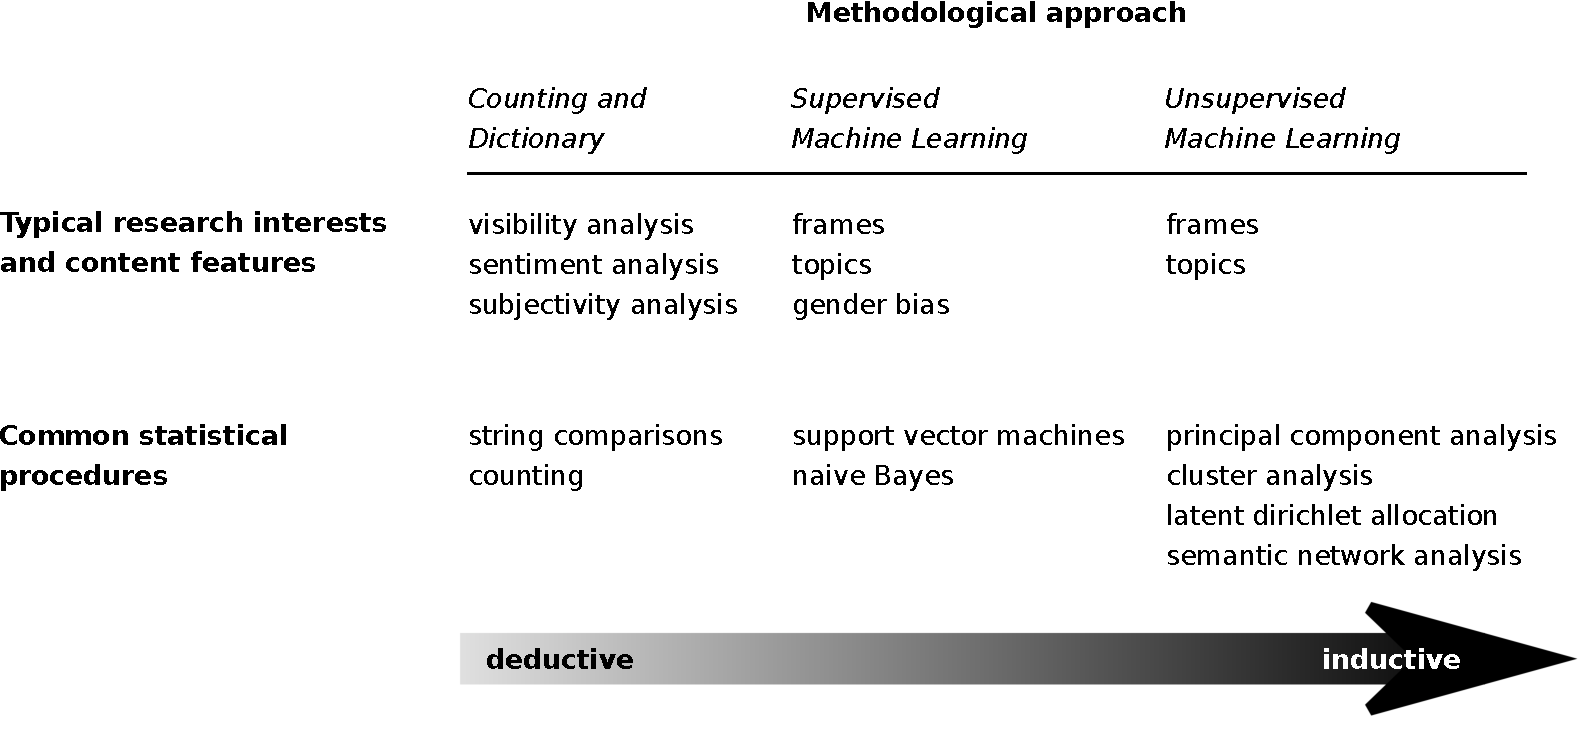
\includegraphics[width=\paperwidth,height=\paperheight,keepaspectratio]{boumanstrilling2016}}
%\cite{Boumans2016}
%
%\textbf{\textcolor{orange}{The same logic applies to non-textual data!}}
%\end{frame}









\begin{frame}{Some terminology }
\begin{columns}[t]
\column{.5\textwidth}

\begin{block}<1-4>{Supervised machine learning}
  You have a dataset with both predictor and outcome (independent and dependent variables; features and labels) --- a \emph{labeled} dataset.
  \onslide<2>{
    \footnotesize{Think of regression: You measured \texttt{x1}, \texttt{x2}, \texttt{x3} and you want to predict \texttt{y}, which you also measured}}
\end{block}

\column{.5\textwidth}

\begin{block}<3->{Unsupervised machine learning}
  You have no labels. \onslide<4>{(\footnotesize{You did not measure \texttt{y})}}\\
  \onslide<5>{\textbf{You might already know \emph{some} techniques to figure out whether \texttt{x1}, \texttt{x2},\ldots \texttt{x\_i} co-occur} \begin{itemize}
    \item Principal Component Analysis (PCA) and Singular Value Decomposition (SVD)
    \item Cluster analysis
    \item Topic modelling (Non-negative matrix factorization and Latent Dirichlet Allocation)
    \item \ldots
    \end{itemize}}
\end{block}

\end{columns}

\end{frame}


\begin{frame}{Let's distinguish four use cases\ldots}

\begin{enumerate}
\item Finding similar variables (dimensionality reduction) -- unsupervised
\item Finding similar cases (clustering) -- unsupervised
\item Predicting a continous variable (regression) -- supervised
\item Predicting group membership (classification) -- supervised
\end{enumerate}
\end{frame}


\begin{frame}[plain]
\begin{table}[]
\resizebox{\textwidth}{!}{%
\begin{tabular}{lllllll}
& x1 & x2 & x3 & x4 & x5 & y \\
case1 & \ding{110}  & \ding{110}  & \ding{110}  & \ding{110}  & \ding{110} & \ding{110} \\
case2 & \ding{110}  & \ding{110}  & \ding{110}  & \ding{110}  & \ding{110} & \ding{110}\\
case3 & \ding{110}  & \ding{110}  & \ding{110}  & \ding{110}  & \ding{110} & \ding{110}\\
case4 & \ding{110}  & \ding{110}  & \ding{110}  & \ding{110}  & \ding{110} & \ding{110}\\
\end{tabular}%
}
\end{table}
 ~ 
\end{frame}



\begin{frame}[plain]
\begin{table}[]
\resizebox{\textwidth}{!}{%
\begin{tabular}{lllllll}
& \textcolor{orange}{x1} & x2 & \textcolor{orange}{x3}& \textcolor{blue}{x4} & \textcolor{blue}{x5} & \textcolor{gray}{(y)} \\
case1 & \textcolor{orange}{\ding{110}}  & \ding{110}  & \textcolor{orange}{\ding{110}}  & \textcolor{blue}{\ding{110}} & \textcolor{blue}{\ding{110}} & \textcolor{gray}{(\ding{110})} \\
case2 & \textcolor{orange}{\ding{110}}  & \ding{110}  & \textcolor{orange}{\ding{110}}  & \textcolor{blue}{\ding{110}} & \textcolor{blue}{\ding{110}} & \textcolor{gray}{(\ding{110})} \\
case3 & \textcolor{orange}{\ding{110}}  & \ding{110}  & \textcolor{orange}{\ding{110}}  & \textcolor{blue}{\ding{110}} & \textcolor{blue}{\ding{110}} & \textcolor{gray}{(\ding{110})} \\
case4 & \textcolor{orange}{\ding{110}}  & \ding{110}  & \textcolor{orange}{\ding{110}}  & \textcolor{blue}{\ding{110}} & \textcolor{blue}{\ding{110}} & \textcolor{gray}{(\ding{110})} \\
\end{tabular}%
}
\end{table}
Dimensionality reduction: finding similar variables (features)
\end{frame}


\begin{frame}[plain]
\begin{table}[]
\resizebox{\textwidth}{!}{%
\begin{tabular}{lllllll}
& x1 & x2 & x3 & x4 & x5 & \textcolor{gray}{(y)} \\
\textcolor{orange}{case1} & \textcolor{orange}{\ding{110}}  & \textcolor{orange}{\ding{110}}  &\textcolor{orange}{\ding{110}}  &\textcolor{orange}{\ding{110}}   & \textcolor{orange}{\ding{110}} & \textcolor{gray}{(\ding{110})} \\
\textcolor{blue}{case2} & \textcolor{blue}{\ding{110}}  & \textcolor{blue}{\ding{110}}  &\textcolor{blue}{\ding{110}}  &\textcolor{blue}{\ding{110}}   & \textcolor{blue}{\ding{110}} & \textcolor{gray}{(\ding{110})} \\
\textcolor{orange}{case3} & \textcolor{orange}{\ding{110}}  & \textcolor{orange}{\ding{110}}  &\textcolor{orange}{\ding{110}}  &\textcolor{orange}{\ding{110}}   & \textcolor{orange}{\ding{110}} & \textcolor{gray}{(\ding{110})} \\
\textcolor{orange}{case4} & \textcolor{orange}{\ding{110}}  & \textcolor{orange}{\ding{110}}  &\textcolor{orange}{\ding{110}}  &\textcolor{orange}{\ding{110}}   & \textcolor{orange}{\ding{110}} & \textcolor{gray}{(\ding{110})} \\
\end{tabular}%
}
\end{table}
Clustering: finding similar cases
\end{frame}



\begin{frame}[plain]
\begin{table}[]
\resizebox{\textwidth}{!}{%
\begin{tabular}{llllllll}
& x1 & x2 & x3 & x4 & x5 & $\rightarrow$ & \textcolor{orange}{y} \\
case1 & \ding{110}  & \ding{110}  & \ding{110}  & \ding{110}  & \ding{110} & $\rightarrow$ &\textcolor{orange}{\ding{110}}  \\
case2 & \ding{110}  & \ding{110}  & \ding{110}  & \ding{110}  & \ding{110} & $\rightarrow$ &\textcolor{orange}{\ding{110}} \\
case3 & \ding{110}  & \ding{110}  & \ding{110}  & \ding{110}  & \ding{110} & $\rightarrow$ &\textcolor{orange}{\ding{110}} \\
case4 & \ding{110}  & \ding{110}  & \ding{110}  & \ding{110}  & \ding{110} & $\rightarrow$ &\textcolor{orange}{\ding{110}} \\
&&&&&&& \\
new case & \ding{110}  & \ding{110}  & \ding{110}  & \ding{110}  & \ding{110} & $\rightarrow$ &\textbf{\textcolor{orange}{?}} \\
\end{tabular}%
}
Regression and classification: learn how to predict $y$.
\end{table}
\end{frame}




\begin{frame}[plain]
\textbf{Note, again, that the \ding{110} signs can be \emph{anything}}: a person's age, the frequency of a word, the color of a pixel, a number of clicks.

\begin{table}[]
\resizebox{\textwidth}{!}{%
\begin{tabular}{lllllll}
& x1 & x2 & x3 & x4 & x5 & y \\
case1 & \ding{110}  & \ding{110}  & \ding{110}  & \ding{110}  & \ding{110} & \ding{110} \\
case2 & \ding{110}  & \ding{110}  & \ding{110}  & \ding{110}  & \ding{110} & \ding{110}\\
case3 & \ding{110}  & \ding{110}  & \ding{110}  & \ding{110}  & \ding{110} & \ding{110}\\
case4 & \ding{110}  & \ding{110}  & \ding{110}  & \ding{110}  & \ding{110} & \ding{110}\\
\end{tabular}%
}
\end{table}
\end{frame}





\section[Predicting things] {Supervising Machine Learning: Predicting things}






\subsection{You have done it before!}
\begin{frame}{You have done it before!}
	\begin{block}{Regression}<2->
		\begin{enumerate}
			\item<3-> Based on your data, you estimate some regression equation 	$y_i = \alpha + \beta_1 x_{i1} + \cdots + \beta_p x_{ip} + \varepsilon_i$
			\item<4-> Even if you have some \emph{new unseen data}, you can estimate your expected outcome $\hat{y}$!
			\item<5-> Example: You estimated a regression equation where $y$ is newspaper reading in days/week: $y = -.8 + .4 \times man + .08 \times age$
			\item<6-> You could now calculate $\hat{y}$ for a man of 20 years and a woman of 40 years -- \emph{even if no such person exists in your dataset}: \\
			$\hat{y}_{man20} = -.8 + .4 \times 1 + .08 \times 20 = 1.2$ \\
			$\hat{y}_{woman40} = -.8 + .4 \times 0 + .08 \times 40 = 2.4$
		\end{enumerate}
	\end{block}	
	
\end{frame}



\begin{frame}{}
	\huge{This is\\ Supervised Machine Learning!}
\end{frame}

\begin{frame}{\ldots but\ldots}
	\begin{itemize}
		\item<1-> We will only use \emph{half} {\tiny{(or another fraction)}} of our data to estimate the model, so that we can use the other half to check if our predictions match the manual coding (``labeled data'',``annotated data'' in SML-lingo)
		\begin{itemize}
			\item<2->e.g., 2000 labeled cases, 1000 for training, 1000 for testing --- if successful, run on 100,000 unlabeled cases
		\end{itemize}
		\item<3-> We use many more independent variables (``features'')
		\item<4-> For text analysis, IVs can be, e.g., word frequencies
	\end{itemize}
\end{frame}


\subsection{From regression to classification}
	
\begin{frame}[standout]
In the machine learning world, predicting some continous value is referred to as a \textcolor{orange}{regression} task. If we want to predict a binary or categorical variable, we call it a \textcolor{orange}{classification} task.

(quite confusingly, even if we use a logistic regression for the latter)
\end{frame}


\begin{frame}{Classification tasks}
For many computational approaches, we are actually not that interested in predicting a continous value. Typical questions include:
\begin{itemize}
	\item Is this article about topic A, B, C, D, or E?
	\item Is this review positive or negative?
	\item Does this text contain frame F?
	\item Is this satire? 
	\item Is this misinformation?
	\item Given past behavior, can I predict the next click?
\end{itemize}
\end{frame}



\begin{frame}[plain]
	\begin{columns}[]
		\column{.5\textwidth}
		
		{\tiny{http://commons.wikimedia.org/wiki/File:Precisionrecall.svg}}
		\makebox[\linewidth]{
			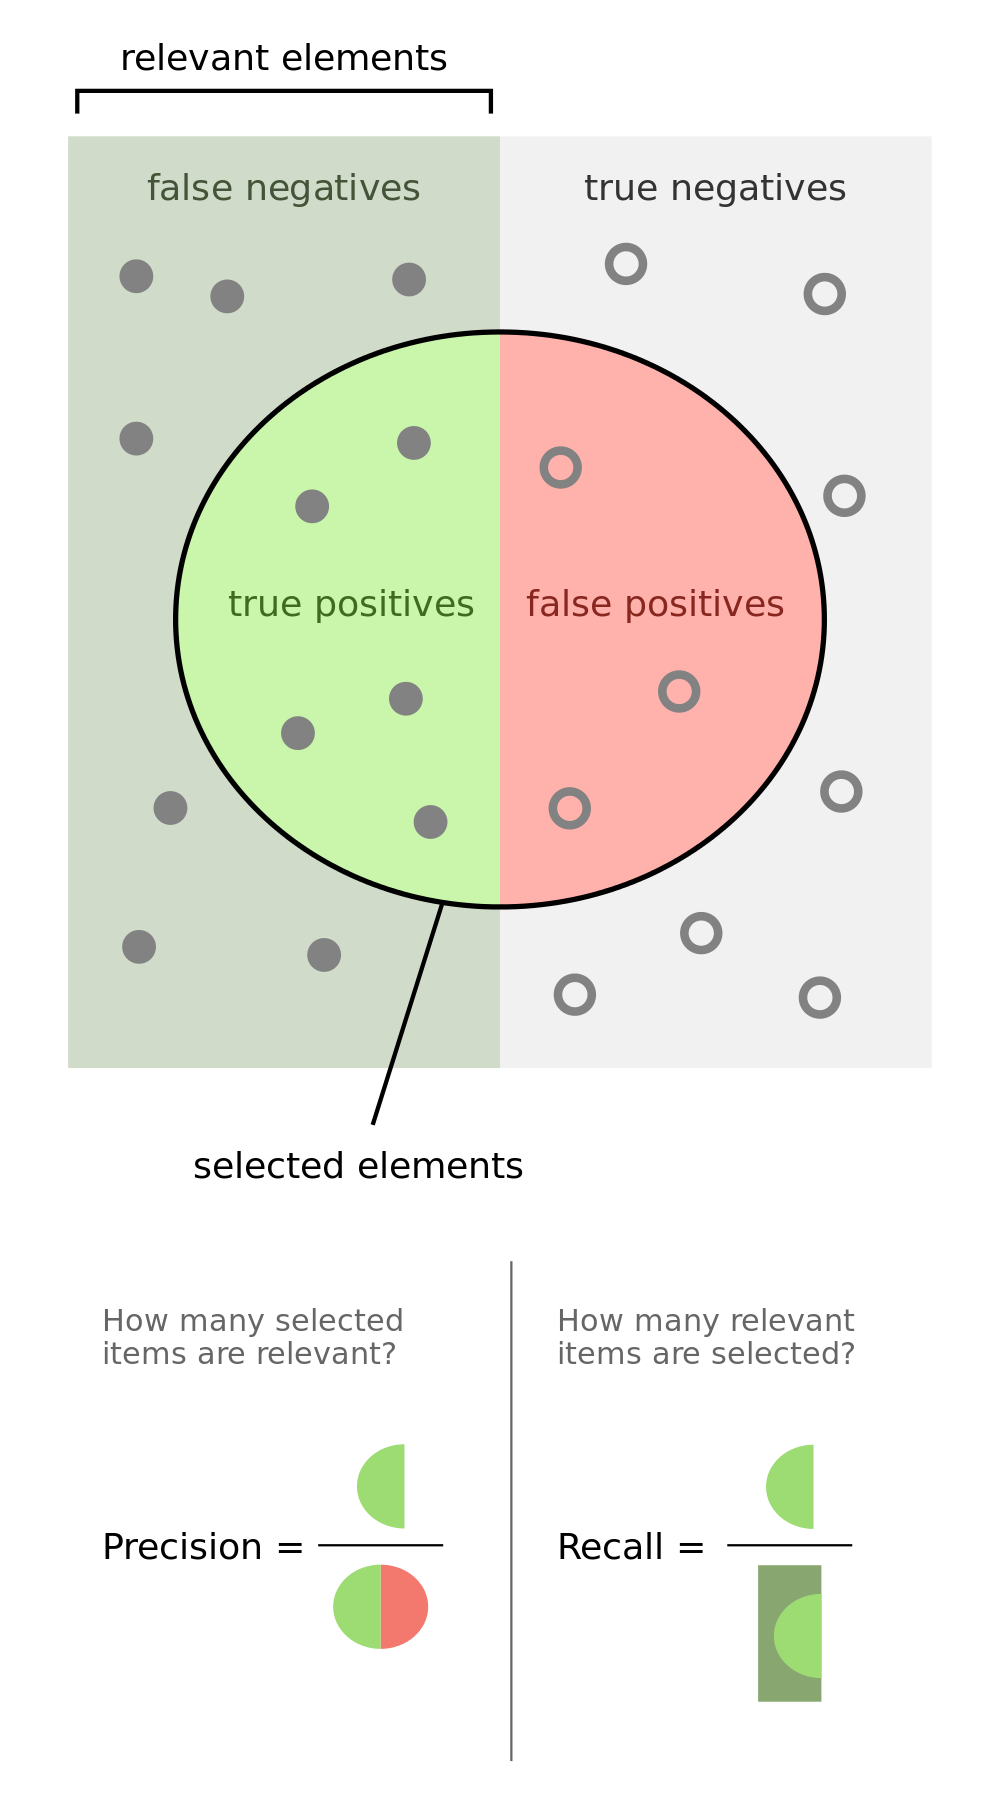
\includegraphics[width=\paperwidth,height=\paperheight,keepaspectratio]{precisionrecall.png}}
		
		\column{.5\textwidth}
		\begin{block}{Some measures}
			\begin{itemize}
				\item Accuracy
				\item Recall
				\item Precision
				\item $\text{F1}=2\cdot \frac{\text{precision}\cdot \text{recall}}{\text{precision}+\text{recall}}$
				\item AUC (Area under curve) $[0,1]$, $0.5=$ random guessing
			\end{itemize}
		\end{block}
		
		
	\end{columns}
	
\end{frame}





\begin{frame}{Different classification algorithms}

\begin{itemize}[<+->]
	\item It is an empirical question which one works best
	\item We typically try several ones and select the best
	\item (remember: we have a test dataset that we did \emph{not} use to train the model, so that we can assess how well it predicts the test labels based on the test features)
	\item To avoid $p$-hacking-like scenario's (which we call ``overfitting''), there are techniques available (cross-validation, later in this course)
\end{itemize}
\pause
To make it easier, we focus on binary classfication (``positive''/``negative''), but it doesn't really matter whether there are two or more labels)
\end{frame}






\begin{frame}{Naïve Bayes}
	\begin{block}{Bayes' theorem}
		$$ P(A \mid B) = \frac{P(B \mid A) \times P(A)}{P(B)} $$
	\end{block}
	\pause
	\textcolor{red}{A = Text is about sports\\
		B = Text contains `very', `close', `game'}.
	\pause
	Furthermore, we simply multiply the propabilities for the features:
	\textcolor{red}{$$P(B) = P(very\, close\, game) = P(very) \times P(close) \times P(game)$$}
	We can fill in all values by counting how many articles are about sports, and how often the words occur in these texts.
	\vspace{0.3cm}
	\tiny{
		(Fully elaborated example on \url{https://monkeylearn.com/blog/practical-explanation-naive-bayes-classifier/})}\\
\end{frame}

\begin{frame}{Naïve Bayes}
	\begin{itemize}[<+->]
		\item It's ``naïve'' because the features are treated as completely independent ($\neq$ ``controlling'' in regression analysis)
		\item It's fast and easy
		\item It's a good \emph{baseline} for binary classification problems
	\end{itemize}
\end{frame}




\begin{frame}{Na\"ive Bayes}
$$ P(\rm{label} \mid \rm{features}) =$$
$$ \frac{P(x_1 \mid label) \cdot P(x_2 \mid \rm{label})\ \cdot P(x_3 \mid label) \cdot P(label)}{P(x_1) \cdot P(x_2) \cdot P(x_3)}$$.

	
\begin{itemize}
	\item Formulas always look intimidating, but we only need to fill in how many documents containing feature $x_n$ have the label, how often the label occurs, and how often each feature occurs
	\item Also for computers, this is \emph{really easy and fast}
	\item Weird assumption: features are independent
	\item Often used as a baseline
\end{itemize}
\end{frame}




\begin{frame}{Logistic Regression}
	\begin{block}{Probability of a binary outcome in a regression model}
		$$p = \frac{1}{1 + e^{-(\beta_0 + \beta_1 x_1 + \beta_2 x_2 + \ldots + \beta_n x_n)}}$$
	\end{block}
	Just like in OLS regression, we have an intercept and regression coefficients. 
	We use a threshold (default: 0.5) and above, we assign the positive label (`good movie'), below, the negative label (`bad movie').
\end{frame}
\begin{frame}{Logistic Regression}
	\begin{itemize}[<+->]
		\item The features are \emph{not} independent.
		\item Computationally more expensive than Naïve Bayes
		\item We can get probabilities instead of just a label
		\item That allows us to say how sure we are for a specific case
		\item \ldots or to change the threshold to change our precision/recall-tradeoff
	\end{itemize}
\end{frame}

\begin{frame}{Support Vector Machines}
	\begin{columns}
		\column{.5\linewidth}
		\begin{itemize}
			\item	Idea: Find a hyperplane that best seperates your cases
			\item Can be linear, but does not have to be (depends on the so-called kernel you choose)
			\item Very popular 
		\end{itemize}
		\column{.5\linewidth}	
		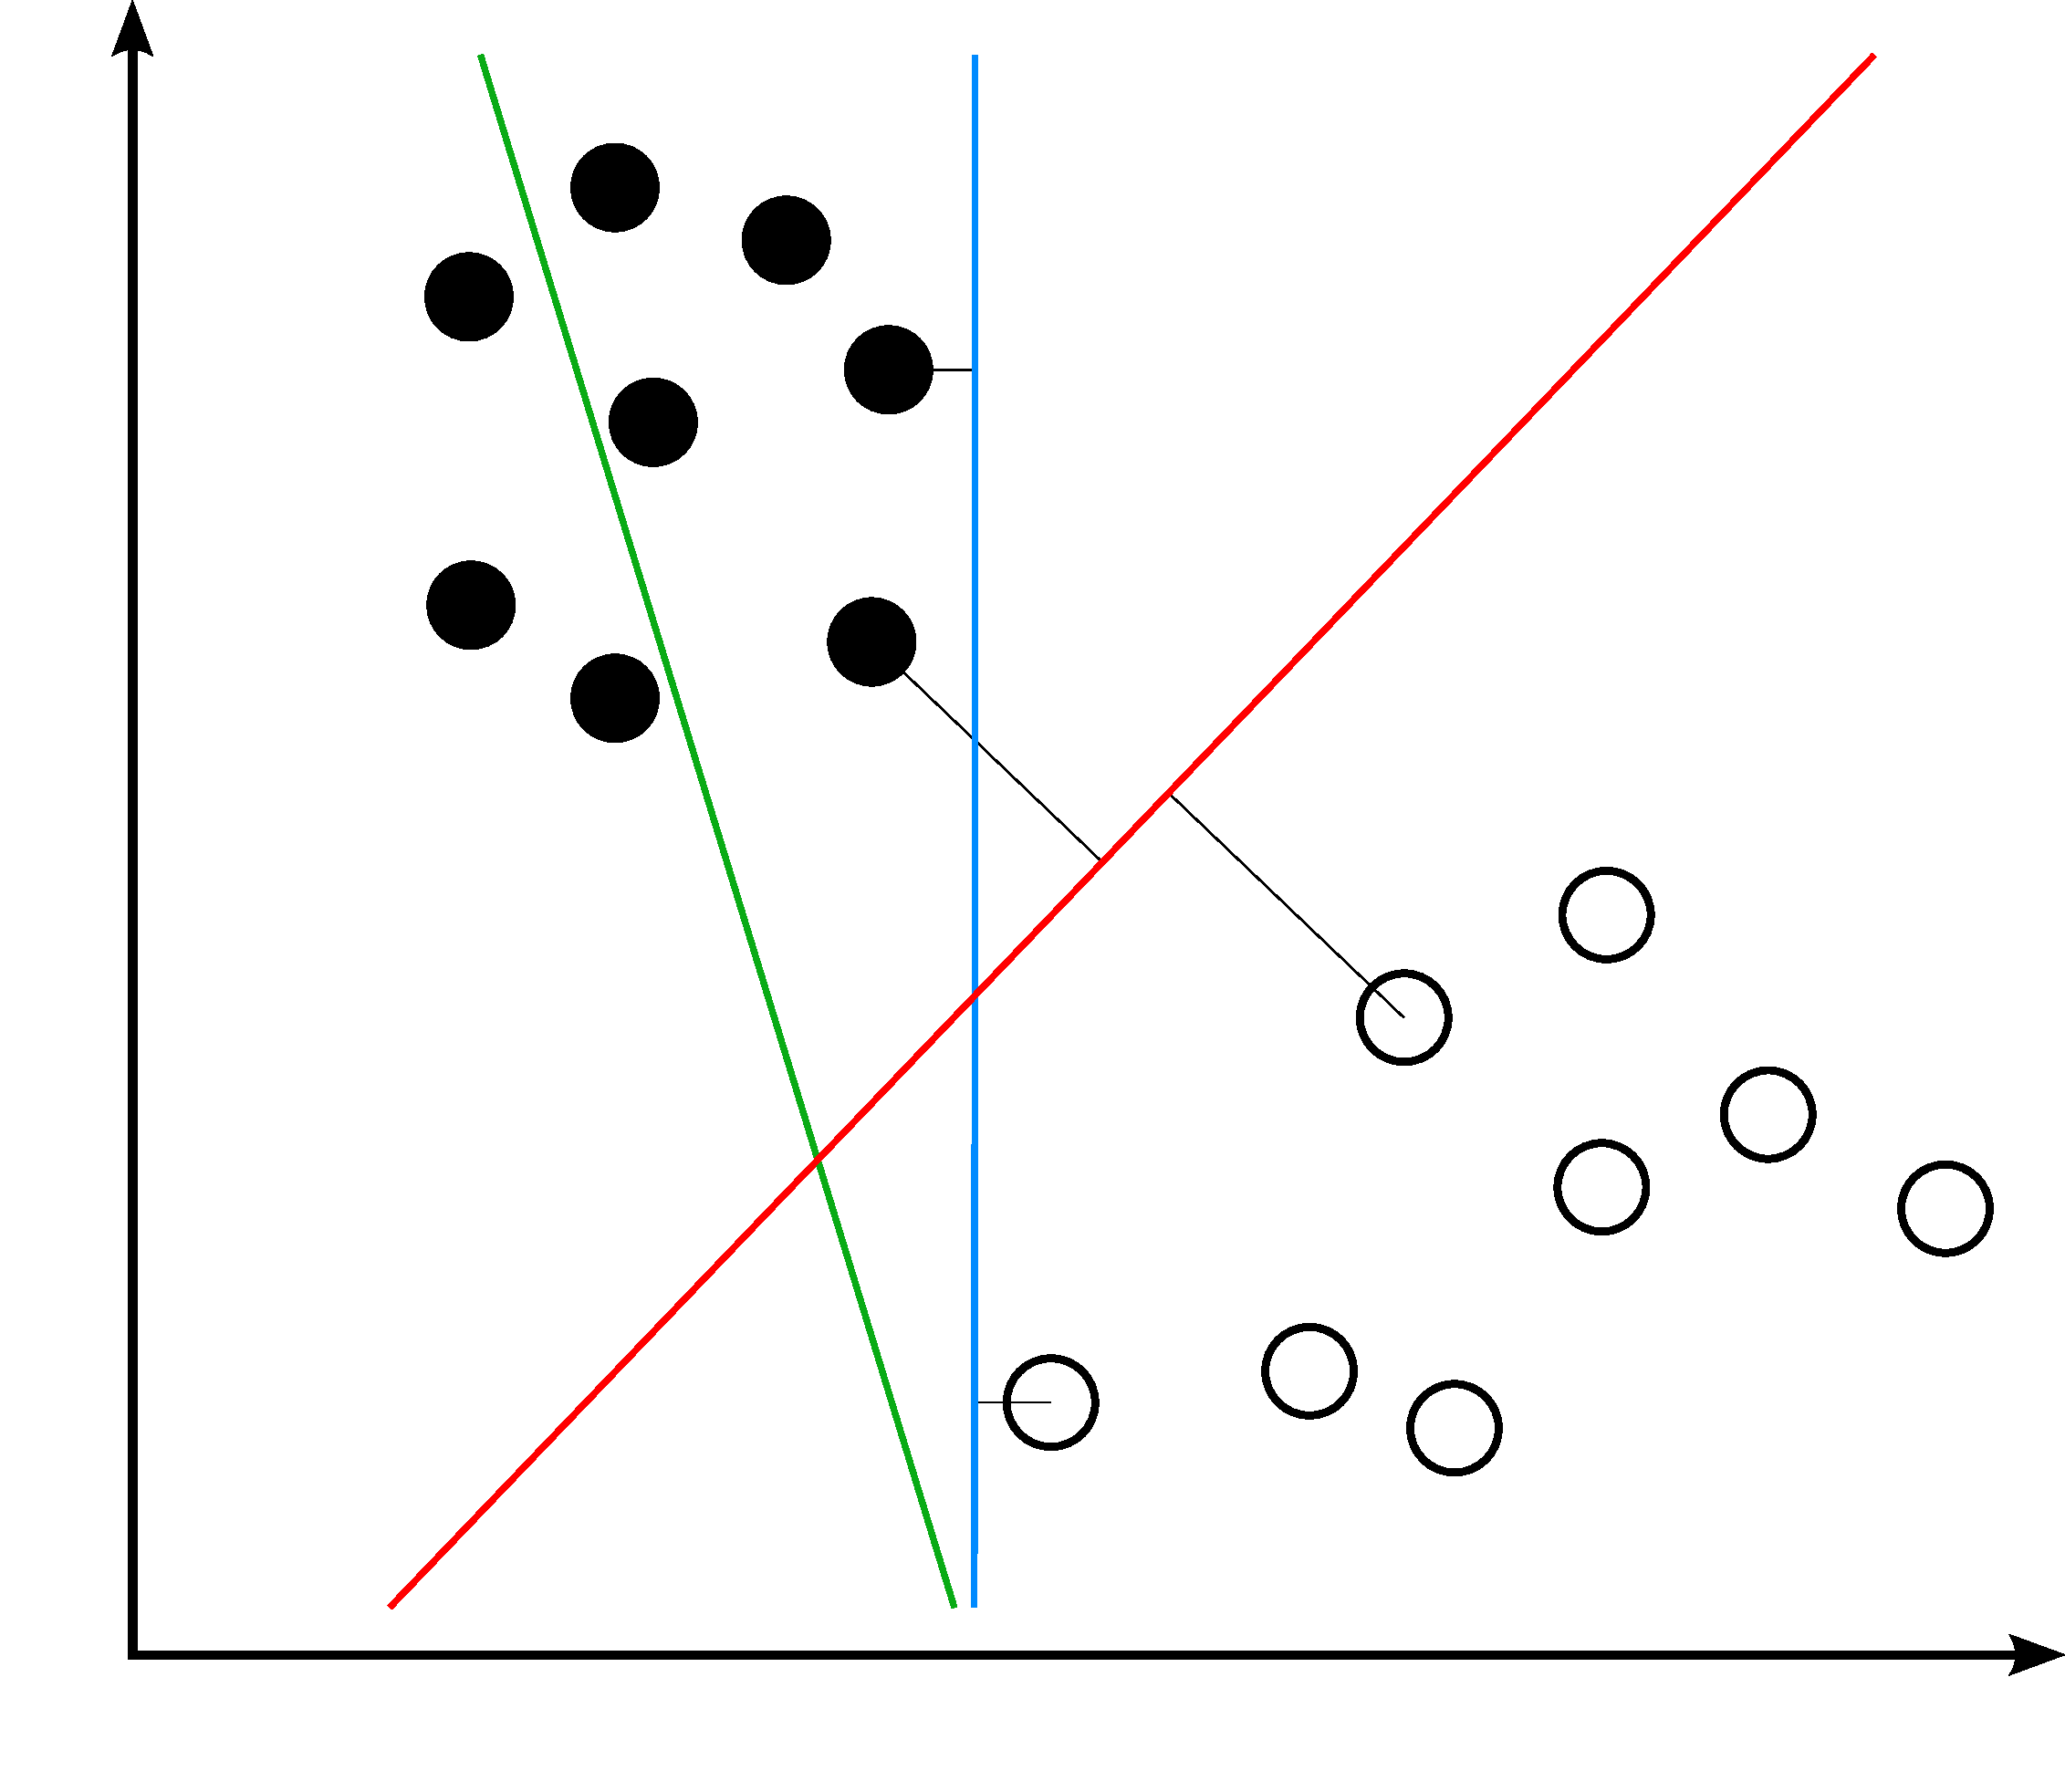
\includegraphics[width=.8\linewidth,height=.5\paperheight,keepaspectratio]{svm}
		\tiny{\url{https://upload.wikimedia.org/wikipedia/commons/b/b5/Svm\_separating\_hyperplanes\_\%28SVG\%29.svg}}
	\end{columns}
	\vfill
	\tiny{(Further reading: \url{https://monkeylearn.com/blog/introduction-to-support-vector-machines-svm/)}}\\
\end{frame}

\begin{frame}{SVM vs logistic regression}
\begin{itemize}
	\item for \emph{linearly separable} classes not much difference
	\item with the right hyperparameters, SVM is less sensitive to outliers
	\item biggest advantage: with the \emph{kernel trick}, data can be transformed that they \emph{become} linearily separable
\end{itemize}
\end{frame}


\begin{frame}{Decision Trees and Random Forests}
  \begin{columns}
    \column{.5\linewidth}
    \begin{itemize}[<+->]
    \item Model problem as a series of decisions (e.g., if cloudy then \ldots if temperature > 30 degrees then \ldots)
    \item Order and cutoff-points are determined by an algorithm
    \item Big advantage: Model non-linear relationships
    \item And: They are easy to interpret (!) (``white box'')
    \end{itemize}
    \column{.5\linewidth}	
		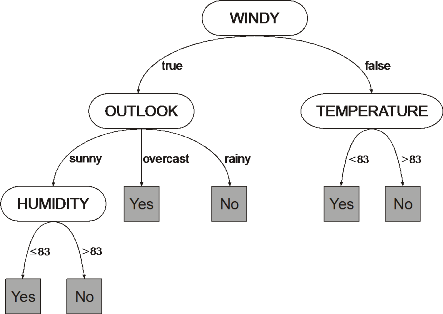
\includegraphics[width=.8\linewidth,height=.5\paperheight,keepaspectratio]{decisiontree}
		\tiny{\url{https://upload.wikimedia.org/wikipedia/en/4/4f/GEP\_decision\_tree\_with\_numeric\_and\_nominal\_attributes.png}}
	\end{columns}
\end{frame}
\begin{frame}{Decision Trees and Random Forests}
  \begin{block}{Disadvantages of decision trees}
    \begin{itemize}
    \item comparatively inaccurate
    \item once you are in the wrong branch, you cannot go `back up'
    \item prone to overfitting (e.g., outlier in training data may lead to completely different outcome)
    \end{itemize}
  \end{block}
  \pause
  Therfore, nowadays people use \emph{random forests}: Random forests \emph{combine} the predictions of \emph{multiple} trees
  $\Rightarrow$ might be a good choice for your non-linear classification problem
\end{frame}


\section[Unsupervised ML]{Unsupervised machine learning}

\begin{frame}{A lot of applications and use cases, \ldots}
\ldots but we'll distinguish two today:

\begin{enumerate}
\item Finding similar variables (dimension reduction)
\item Finding similar cases (clustering)
\end{enumerate}

\pause

Are we more interested in which features ``belong together'' or which cases ``belong together''? 

\emph{There are many other techniques than those presented today, and vice versa, those presented today can also be used for other purposes}

\end{frame}

\subsection{Finding similar variables}

\subsubsection{An introduction to dimensionality reduction}


\begin{frame}{Dimensionality reduction}
dimensionality = the number of features we have
\begin{block}{(1) Explorative data analysis and visualization}
\begin{itemize}
\item No good way to visualize 10,000 dimensions (or even 4)
\end{itemize}
\end{block}

\pause

\begin{block}{(2) The curse of dimensionality}
More features means more data (good!), but:
\begin{itemize}
\item Too many features can lead to unfeasible computation times
\item We need more training cases to increase the likelihood that the possible combinations actually occur
\end{itemize}
\end{block}
\end{frame}



\begin{frame}[fragile]{Dimensionality reduction}

\begin{block}{Feature extraction}
\begin{itemize}
\item Create a smaller set of features
\item E.g.: 1,000 features $\rightarrow$ PCA to reduce to 50 components $\rightarrow$ SML with these 50 component scores as features
\end{itemize}
\end{block}

\end{frame}



\begin{frame}[fragile]{Dimensionality reduction}

So, we can use unsupervised ML as a dimension reduction step in a supervised ML pipeline. 
\vspace{0.5cm}

But it can also be a goal in itself, to understand the data better or to visualize them.
\end{frame}







\subsubsection{Principal Component Analysis and Singular Value Decomposition}


\begin{frame}{PCA}
\begin{itemize}
\item related to and often confused with Factor Analysis (same menu item in SPSS -- many people who believe they run FA actually run PCA!)
\item Components are ordered (first explains most variance)
\item Components do \emph{not} necessarily carry a meaningful interpretation
\end{itemize}
\end{frame}

\begin{frame}{PCA}
\makebox[\linewidth]{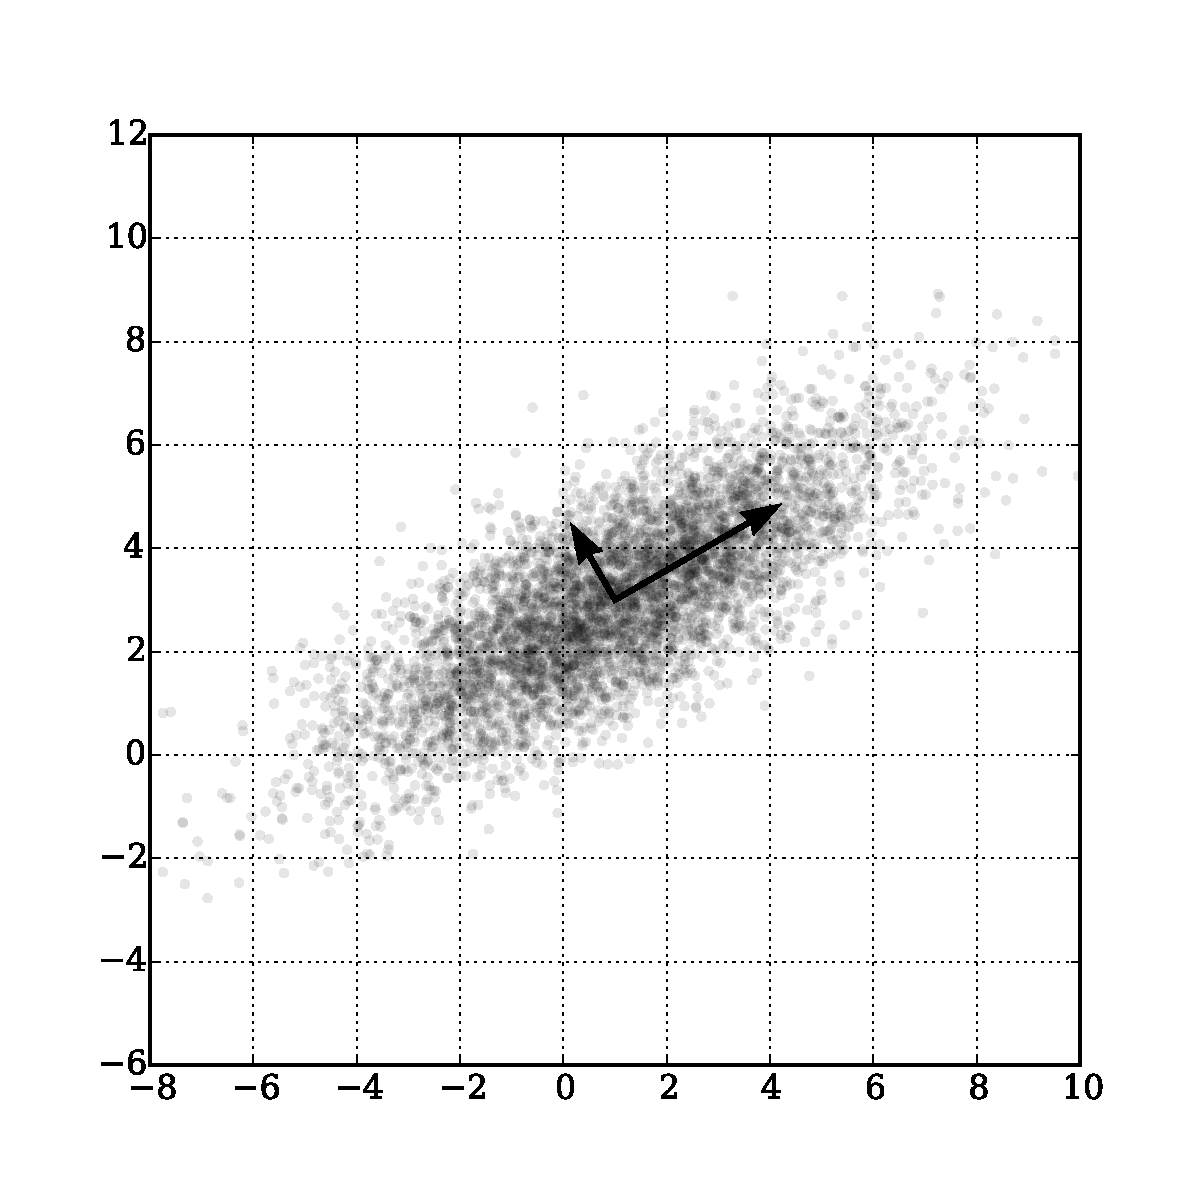
\includegraphics[width=\paperwidth,height=.6\paperheight,keepaspectratio]{pca}}

\tiny{\url{https://upload.wikimedia.org/wikipedia/commons/f/f5/GaussianScatterPCA.svg}}
\end{frame}



\begin{frame}[fragile,plain]{Preparation: Import modules and get some sample data}
\begin{minted}{python}
import pandas as pd
from sklearn.decomposition import PCA
from sklearn.preprocessing import StandardScaler

df = pd.read_csv("https://cssbook.net/d/eurobarom_nov_2017.csv")\
    .dropna()\
    .groupby(["country"])[[
    "support_refugees_n", 
    "support_migrants_n", 
    "age", 
    "educational_n"]].mean()
\end{minted}


\begin{lstlistingoutputtiny}
country   support_refugees_n  support_migrants_n        age  educational_n                                                                
Austria             2.847674            2.576744  49.445349      18.930233
Belgium             2.772619            2.252381  53.002381      19.338095
Bulgaria            2.075159            1.769427  51.517197      19.652229
Croatia             2.717105            2.002193  47.001096      18.899123
Cyprus              3.018141            2.104308  53.734694      18.598639
\end{lstlistingoutputtiny}
\end{frame}






\begin{frame}[fragile,plain]{Running PCA}
  \begin{minted}{python}
# we first standardize our data to z-scores
scaler = StandardScaler()
df_s = scaler.fit_transform(df) 
    
mypca = PCA()
componentscores = mypca.fit_transform(df_s)
scores_df = pd.DataFrame(componentscores, index=df.index)

components_df = pd.DataFrame(data=mypca.components_.T)
components_df.index = df.columns
print("Variable loadings on the 4 components:")
print(components_df)  

# This is the transformed dataset
# As we will see in a minute, we retain 86\% of the
# variance even if we keep only the first 2 components
print("The component scores for each case:")
print(scores_df)
\end{minted}
\end{frame}



\begin{frame}[fragile,plain]{Running PCA}
\begin{lstlistingoutputtiny}
Variable loadings on the 4 components:
                           0         1         2         3
support_refugees_n  0.573292 -0.369010  0.139859  0.718058
support_migrants_n  0.513586 -0.533140 -0.094283 -0.665659
age                 0.445117  0.558601  0.670994 -0.199005
educational_n       0.457642  0.517261 -0.722023  0.041073


The component scores for each country:
                       0         1         2         3
country                                               
Austria        -0.103285 -1.220018 -0.535673  0.066888
Belgium        -0.029355 -0.084707  0.051515  0.227609
Bulgaria       -1.660518  0.949533 -0.480337 -0.151837
Croatia        -1.267502 -0.819093 -0.920657  0.843682
Cyprus          0.060590 -0.195928  0.573670  0.812519
Czech republic -2.219795  0.675655 -0.763679 -0.086147
Denmark         2.925631  1.516636 -0.748940  0.495489
Estonia        -0.602217  2.206418  0.785869 -0.152262
Finland         2.224310  1.384983 -0.169499 -0.468742
France         -0.102062 -0.046415  0.228587 -0.122965
Germany         0.917864 -0.259560  0.940792  0.319158
Greece         -0.832343 -0.313480  0.329525  0.683748
Hungary        -2.234701  0.716823  0.391788 -0.315312
Ireland         0.993243 -1.767147 -0.592957 -0.168892
\end{lstlistingoutputtiny}
\end{frame}









\begin{frame}[fragile,plain]{Plotting the result}
  \begin{minted}{python}
import bioinfokit.visuz
   
bioinfokit.visuz.cluster.biplot(cscore=componentscores, 
  loadings=mypca.components_, 
  labels=df.columns, 
  var1=round(mypca.explained_variance_ratio_[0],2), 
  var2=round(mypca.explained_variance_ratio_[1],2), 
  show=True)  
\end{minted}

\makebox[\linewidth]{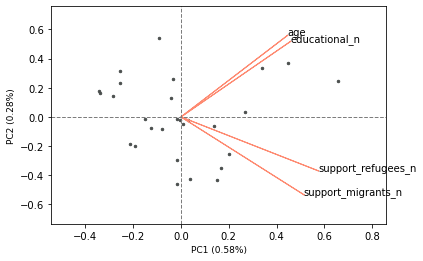
\includegraphics[width=\paperwidth,height=.6\paperheight,keepaspectratio]{pca-example-book}}

\end{frame}



\begin{frame}[fragile,plain]{Plotting the result}
  \begin{minted}{python}
import numpy as np
import matplotlib.pyplot as plt

fig, ax = plt.subplots()
ax.plot(np.cumsum(mypca.explained_variance_ratio_))
ax.set_xticks(range(mypca.n_components_))
ax.set_xticklabels(range(1, mypca.n_components_+1))
ax.set_xlabel("number of components") 
ax.set_ylabel("cumulative explained variance") 
ax.set_ylim(0,1)
fig.savefig("pca-explained-variance.png")   # optional of course
\end{minted}

\makebox[\linewidth]{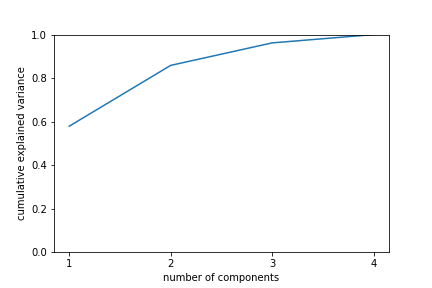
\includegraphics[width=\paperwidth,height=.3\paperheight,keepaspectratio]{pca-explained-variance}}

\end{frame}






\begin{frame}{Singular value decomposition}

\begin{alertblock}{PCA uses a dense matrix!}
In ``real life'' with larger datasets (essentially, everything (!) involving text), we never use PCA but SVD. It works exactly the same (check out \url{scikit-learn.org}), but does not require to hold a dense matrix in memory. Instead, it operates on a sparse matrix, in which only non-zero values are stored. (this will make a lot of sense once we talk about textual data)
\end{alertblock}

  
\footnotesize{
* It's mathematically different, but SVD is even used ``under the hood'' by several PCA modules to solve PCA problems.
More info and background: \url{https://towardsdatascience.com/pca-and-svd-explained-with-numpy-5d13b0d2a4d8}}
\end{frame}







\subsection{Finding similar cases}

\subsubsection{k-means clustering}

\begin{frame}{Grouping features vs grouping cases}
  \begin{itemize}[<+->]
  \item  In the previous example, we established that \emph{age} and \emph{education} measure almost the same thing, and so do \emph{support\_refugees} and \emph{support\_migrants}.
  \item We could now, for instance, check out which countries receive similar scores to group them.
  \item But if grouping countries (instead of variables) is our goal in the first place, we can directly do so.
  \end{itemize}
\end{frame}




\begin{frame}{k-means clustering}
\begin{itemize}[<+->]
\item Goal: group cases into $k$ clusters
\item $k$ is set in advance
\item Algorithm to determine \textit{k} centroids (points in the middle of the cases that belong to it) such that the distances between the cases and their centroids are minimized
\item non-deterministic: starts with a randomly choosen centroids (there are other versions)
\item Cheap to compute: works even with large number of cases
\item We can run PCA first to reduce the number of features if we want/need to
\end{itemize}
\end{frame}




\begin{frame}{k-means clustering}
\makebox[\linewidth]{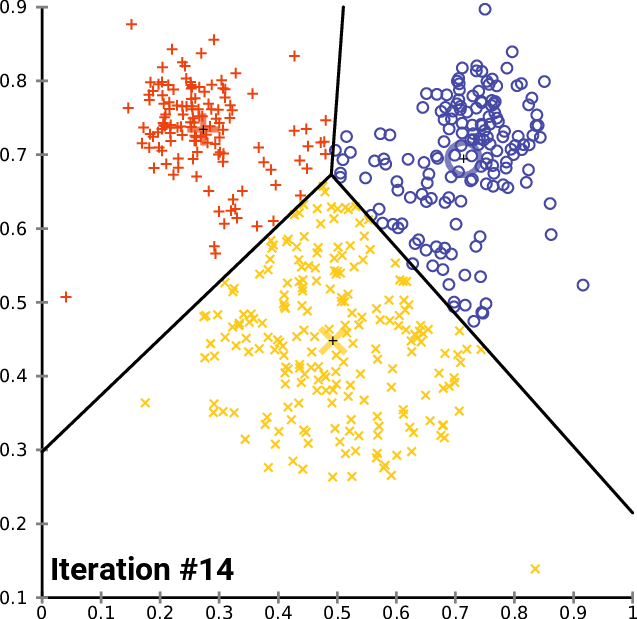
\includegraphics[width=\paperwidth,height=.65\paperheight,keepaspectratio]{kmeans}}

{\tiny{\url{https://upload.wikimedia.org/wikipedia/commons/e/ea/K-means\_convergence.gif}}}

Notice the big symbols indicating the centroids.
\end{frame}


\begin{frame}[plain,fragile]
\begin{lstlisting}
from sklearn.cluster import KMeans

# everything needs to be measured on the same scale,
# therefore we take the scaled dataset

mykm = KMeans(n_clusters=3).fit(df_s)
pd.DataFrame({"country":df.index, "cluster":mykm.labels_})
\end{lstlisting}

\begin{lstlistingoutputtiny}
           country  cluster
0          Austria        1
1          Belgium        1
2         Bulgaria        0
3          Croatia        0
4           Cyprus        1
5   Czech republic        0
\end{lstlistingoutputtiny}

\end{frame}



\begin{frame}{Finding the optimal $k$}

\begin{itemize}
\item The only way to find $k$ is to estimate multiple models with different $k$s
\item No single best solution; finding a balance between error within clusters (distances from centroid) and low number of clusters.
\item An elbow plot can be helpful
\end{itemize}
\end{frame}


\begin{frame}[fragile,plain]{Finding the optimal $k$}
\begin{minted}{python}
wss = []
for i in range(1, 15):
    km = KMeans(n_clusters=i)
    km.fit(df_s)
    wss.append(km.inertia_)

fig, ax = plt.subplots()
ax.plot(range(1, 15), wss, marker="o")
ax.set_xlabel("Number of clusters")
ax.set_ylabel("Within groups sum of squares")
\end{minted}

\makebox[\linewidth]{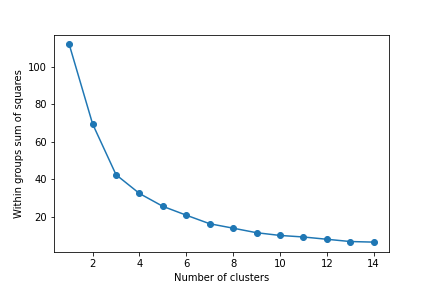
\includegraphics[width=\paperwidth,height=.3\paperheight,keepaspectratio]{kmeans-elbow}}

\end{frame}





\subsubsection{Hierarchical clustering}

\begin{frame}{Downsides of k-means clustering}
k-means is fast, but has problems:

\begin{itemize}
\item $k$ can only be determined by fitting multiple models and comparing them
\item bad results if the wrong $k$ is chosen
\item bad results if the (real) clusters are non-spherical
\item bad results if the (real) clusters are not evenly sized
\end{itemize}
\end{frame}


\begin{frame}{Hiearchical clusttering}
\begin{block}{General idea}
\begin{itemize}
\item To start, each case has its own cluster
\item Merge the two clusters that are most similar
\item Repeat until desired number of clusters is reached
\end{itemize}

\end{block}

\pause

\begin{block}{Different options}
\begin{itemize}
\item Stopping criterion: based on numerical statistic (e.g., Duda-Hart) or dendrogram
\item Linkage: how to determine which two clusters should be merged?
\end{itemize}

\end{block}
\end{frame}


\begin{frame}{Let's look into some options}

\url{https://scikit-learn.org/stable/modules/clustering.html\#hierarchical-clustering}

$\Rightarrow$ Ward's linkage is a good default all-rounder choice, especially if you encounter the problem that other linkages lead to almost all cases ending up in one cluster. 
\end{frame}


\begin{frame}{Hierarchical clustering takeaway}
\begin{itemize}
\item The main reason \emph{not} to use hierarchical methods (but k-means) is their computational cost: when clustering survey data of media users, never use $k$-means!
\item But for NLP/ML, costs may be too high (if not used carefully)
\item Very much worth considering, though, if you are really into grouping cases!
\end{itemize}
\end{frame}


\begin{frame}{Important notes (for \emph{all} techniques today)}
\begin{block}{Consider the scales of measurement}
Clustering is based on distances -- if your features are not measured on the same scale, or if it is not meaningful to calculate a numerical distance, it won't produce meaningful results!

Consider standardizing/whitening your features!
\end{block}

\pause

\begin{block}{Pay attention outliers/extreme cases}
Extreme cases or outliers can have a strong influence.
\end{block}

\pause 
\begin{block}{Do proper pre-processing}
To reduce the number of features, but also to have \emph{meaningful} features (dimensions on which you expect high distances between the clusters).
\end{block}


\end{frame}












\question{Any questions?}

\section{Next steps}

\begin{frame}[standout]
Make sure you understood all of today's concepts.

Re-read the chapters.

I prepared exercises to work on \emph{during} the Friday meeting (alone or in teams):
\large{\url{https://github.com/uvacw/teaching-bdaca/blob/main/12ec-course/week04/exercises/}}
\end{frame}


\begin{frame}[standout]
Take-home exam next week Friday!
\end{frame}





\begin{frame}[allowframebreaks,plain]
	\printbibliography
\end{frame}



\end{document}
